\documentclass[handout]{beamer}
\mode<presentation>{\usetheme{Warsaw}\usecolortheme{crane}}
\usepackage{centernot}
\usepackage{graphicx}

\usepackage[utf8]{inputenc}
\usepackage[english]{babel}
\usepackage{lmodern}
\usepackage[T1]{fontenc}
\usepackage[babel=true]{microtype}

%% preamble
\title{UNIX Weapons School---Introduction}
\subtitle{{\it Lasciate ogni speranza, voi ch'entrate!}}
\date{}
\author{Nick Black for the\\
Georgia Institute of Technology
}

\begin{document}

\begin{frame}
\titlepage
\begin{center}

\includegraphics[scale=0.33]{uws.png}
\end{center}
\end{frame}

\begin{frame}{High-Level Goals}
\begin{itemize}
\item Train formidably competent systems programmers.
\item Ensure GT continues to graduate world-class hackers.
\item Provide a fast-paced challenge for talented, driven students. 
\item Inculcate a profound appreciation of performance.
\end{itemize}
\end{frame}

\begin{frame}{Low-Level Goals}
\begin{itemize}
\item Introduce a collection of UNIX development tools.
\item Introduce advanced algorithms and data structures.
\item Demonstrate analysis-driven optimization.
\item Survey the modern x86 instruction set and UNIX kernel.
\end{itemize}
\end{frame}

\begin{frame}{Unofficial Goals}
\begin{itemize}
\item Establish a historical perspective on computer science.
\item Foster a respect for and devotion to open source.
\item Churn out desirable job candidates.
\end{itemize}
\end{frame}

\begin{frame}{Assumptions}
\begin{itemize}
\item You are not required to take this class.
\uncover<2->{
\begin{itemize}
\item This assumption is also an answer to most complaints.
\item Hopefully you represent a self-selection of the elite.
\end{itemize}
}
\item You are dexterous with C.
\uncover<3->{
\begin{itemize}
\item You ought be able to pump out working C pretty quickly...
\item ... and be able to recognize any C construct.
\item A copy of {\it The C Programming Language} is recommended.
\end{itemize}
}
\item You have a 64-bit x86 Linux box readily available.
\uncover<4->{
\begin{itemize}
\item I can't {\it require} you to install Linux, but...
\item You're CS majors. Why aren't you running open source?
\item We will regularly refer to and modify GNU/Linux source code.
\end{itemize}
}
\end{itemize}
\end{frame}

\begin{frame}{Relation to CoC I}
UWS relies upon and extends:
\begin{itemize}
\item CS2110 (Bill Leahy) -- C-based systems
\item CS35xx (Dr. STAFF) -- Algorithms
\item CS325x (Dr. STAFF) -- Networking
\end{itemize}
UWS borrows material from:
\begin{itemize}
\item CS6230 (Richard Vuduc) -- HPC Tools and Methods
\item CS6290 (Hyesoon Kim / Milos Prvulovic) -- Comp Arch
\item CS6251 (Santosh Pande) -- Compiler Design
\item Whatever Tom Conte's teaching at the moment
\end{itemize}
\end{frame}

\begin{frame}{Relation to CoC II}
but... \\
\emph{UWS focuses on {\it use} of these theories to produce high-performance,
robust, {\it practical} system software solutions.}\linebreak \\
e.g.: \\
You will not gain experience implementing SSA (single static
assignment, which if you don't know now, you'll know later), but you will
understand the space of optimizations an SSA-driven compiler can effect on your
code.\linebreak \\
{\bf UWS will involve writing \~{}10,000 lines of code.}\linebreak \\
This is Sparta, young friends. Feel free to leave.
\end{frame}

\begin{frame}{Projects I}
Four variably-weighted projects compose the entirety of your grade:
\vspace{.25in}
\begin{itemize}
\item A high-performance, lock-free allocator
\item A parallel DFA/regular expression engine
\item A dynamic ELF binary instrumentation tool
\item An event-driven compute transaction engine
\end{itemize}
\vspace{.25in}
This list is subject to change.\\
\begin{figure}[b!]
\hfill 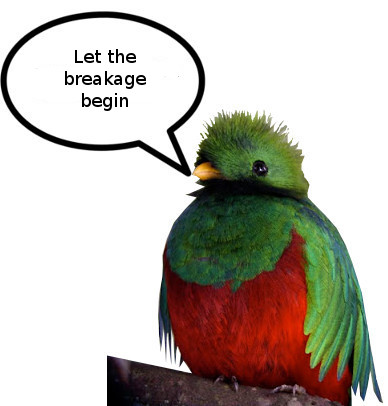
\includegraphics[scale=0.33]{breakage.jpg}
\end{figure}
\end{frame}

\begin{frame}{Projects II}
\begin{itemize}
\item There are no teams, but you may discuss the project freely among
	yourselves.
\item We will not discuss the projects in class, but they will be
	covered at length on the mailing list.
\item Your internal design freedom is total\footnote{Save contact of off-system oracles, which is prohibited.};\\
your external design freedom is nil.
\item You will have access to reference platforms on which your code will be
	(automatically) tested.
\end{itemize}
\end{frame}

\begin{frame}{Cheating}
\begin{center}
If you cheat, I will set you on fire.
\vspace{.5in}

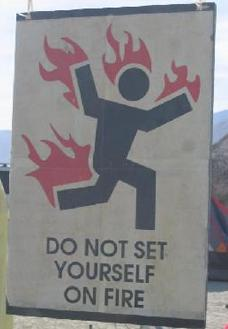
\includegraphics[scale=0.5]{setonfire.jpg}
\end{center}
\end{frame}

\begin{frame}{Project Grading}
\begin{itemize}
\item I will prepare $U$, unit tests for each assignment $A_0 \dotsc A_3$.
\item For each assignment $A_a$, for each unit test $U_{a_j}$
\begin{itemize}
\item Invoke turnin $T_{a_{i \in S}}$ upon $U_{a_j}$ in a clean environment
\item Sort $|C_u|$ correct projects $0 \dotsc n\ge 0$ by decreasing running time
\item If $|C_u| = 1$, award 1.5 points to turnin $T_{a_i} \in C_u$, otherwise
\begin{equation}
\forall i \forall j, T_{a_i} = C_{u_j} \implies \text{award } \frac{j}{|C_u| - 1} \text{ points to } T_{a_i}
\nonumber
\end{equation}.
\item NB: The slowest of multiple correct projects receives 0 points.
\end{itemize}
\item Total points awarded = your score for the project.
\end{itemize}
\end{frame}

\begin{frame}{Semester Grading}
Project scores are totaled yielding $\{p_0, p_1, \dotsc p_{|S| - 1}\}$.\linebreak \\
$G(p)$ maps $p$ to $\{A > B > C > D \cong F\}$ such that\footnote{Either the ``grading function'' or ``Greenlee function''.}
\begin{equation}
\forall i \forall j, p_i > p_j \implies G(p_i) \ge G(p_j), \nonumber
\end{equation}
\begin{equation}
\forall i \forall j, p_i = p_j \implies G(p_i) = G(p_j), \nonumber \linebreak
\end{equation}
\begin{equation}
\forall i \forall j, p_i\gg p_j \centernot\implies G(p_i) > G(p_j) \nonumber
\end{equation}
subject to:
\begin{equation}
\forall i, G(p_i) = \{A, D, F\} \implies S_i\ \text{really deserved it}\nonumber
\end{equation}
with non-binding expectations:
\begin{equation}
|G_D| = 0 \le |G_F| < |G_A| < \frac{|G_B|}{e} \simeq \frac{|G_C|}{e} \nonumber
\end{equation}
\end{frame}

\begin{frame}{Introibimus ad altare Dei---our adventure begins!}
\begin{center}
Let us go then, you and I.

\vspace{.25in}
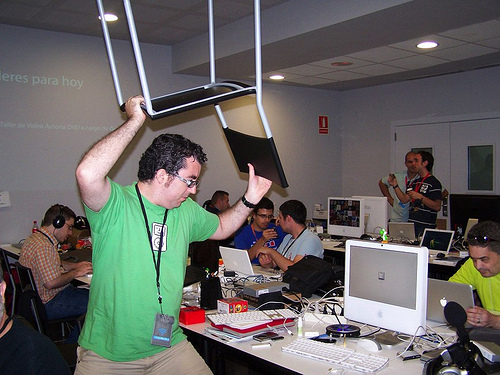
\includegraphics[scale=0.33]{angry.jpg}
\vspace{.25in}

'Tis not too late to seek a newer world.
\end{center}
\end{frame}

\end{document}
